\documentclass[11pt]{article}

% Camera-ready (non-anonymous, no line numbers, no page numbers).
% Change "acl" to "[review]{acl}" to regenerate the anonymous review version.
\usepackage{acl}

\usepackage{times}
\usepackage{latexsym}
\usepackage[T1]{fontenc}
\usepackage[utf8]{inputenc}
\usepackage{microtype}
\usepackage{inconsolata}
\usepackage{graphicx}
\usepackage{booktabs}
\usepackage{amsmath}
\usepackage{amssymb}
\usepackage{multirow}
\usepackage{xcolor}
\usepackage{orcidlink}

% Figures live one level up
\graphicspath{{../figures/}}

% Convenience: highlight items pending verification
\newcommand{\verify}[1]{\textcolor{red}{[VERIFY: #1]}}

% ---------------------------------------------------------------
\title{Thought Anchors for Social Bias: Which Reasoning Steps Matter\\
in Extended Thinking LLMs on Latin American Scenarios}

\author{Andres Mosquera-Hernandez\,\orcidlink{0009-0009-3882-2169} \\
  Systems and Computing Engineering Department \\
  Universidad de Los Andes \\
  Cra.\ 1E No.\ 19A-40, Bogotá, Colombia \\
  \texttt{a.mosquerah2@uniandes.edu.co} \\}
% ---------------------------------------------------------------

\begin{document}
\maketitle

% ---------------------------------------------------------------
\begin{abstract}
We investigate which reasoning steps in extended-thinking LLMs are
associated with pro-stereotypical outputs on Latin American social
bias scenarios. Social bias benchmarks, including BBQ
\citep{parrish2022bbq}, SESGO \citep{robles2024sesgo}, and
EsBBQ/CaBBQ \citep{ruizfernandez2025esbbq}, measure final-answer
distributions but provide no visibility into intermediate reasoning.
We adapt the thought-anchor resampling framework
\citep{bogdan2025thoughtanchors} to social bias measurement: for each
sentence-level chunk in a model's chain-of-thought, we remove it,
resample $K{=}3$ continuations, and measure the change in
pro-stereotypical output probability via three importance metrics.
We apply this pipeline to SESGO-small, an 80-item stratified pilot
subset spanning four Latin American bias categories
(\textit{género, clasismo, racismo, xenofobia}), two languages, and
three recent models with extended thinking.
Across 1,708 chunk-level attributions, disambiguated contexts show
higher pro-stereotypical output rates than ambiguous ones
(33–75\% vs.\ 0\%), and high-importance
reasoning positions tend to be tagged as \texttt{logical\_reasoning}
or \texttt{context\_recall} rather than \texttt{stereotype\_activation}.
These pilot results suggest that bias-relevant moments may lie in
general inference steps rather than overt stereotype invocations,
offering a step-level diagnostic target that complements answer-level
benchmarks.
More broadly, attributing bias to specific reasoning steps could help
localize where stereotyping enters a model's reasoning, though our
findings remain preliminary.
\end{abstract}

% ---------------------------------------------------------------
\section{Introduction}

Extended-thinking LLMs now expose their chain-of-thought as a separable
reasoning stream produced before the final answer. This capability
opens a question that prior bias evaluations cannot address: at which
specific reasoning step does a model tend toward a stereotypical output?

Social bias benchmarks have documented that LLMs produce stereotypical
final answers across cultural contexts: BBQ \citep{parrish2022bbq} for
the United States, SESGO \citep{robles2024sesgo} for Latin America,
CBBQ \citep{huang2023cbbq} for China, and KoBBQ \citep{jin2024kobbq}
for Korea. Despite this progress, all operate at the final-answer level.
B-score \citep{vo2025bscore} extends evaluation to multi-turn patterns
but still measures answer-level phenomena. The thought-anchor framework
\citep{bogdan2025thoughtanchors} assigns importance scores to
individual chain-of-thought steps for mathematical reasoning, but has
not been applied to social bias.
The result is a gap: it remains unclear whether biased outputs tend to
arise at explicit stereotype invocations, at general logical inference
steps, or at the moment of option evaluation.

We take a step toward closing this gap by adapting thought-anchor
resampling to social bias measurement on SESGO. Our contributions are:

\begin{itemize}
  \item \textbf{Step-level bias attribution pipeline.} We adapt
    thought-anchor resampling to produce chunk-level importance scores
    for stereotypical reasoning in extended-thinking LLMs, a granularity
    not addressed by prior bias benchmarks, to our knowledge.

  \item \textbf{Pilot evidence for the disambiguation effect.}
    On SESGO-small, pro-stereotypical output rates are higher in
    disambiguated contexts (33–75\%) than ambiguous contexts
    (0\%) across all three evaluated models, consistent with the core
    BBQ finding in a multilingual Latin American setting.

  \item \textbf{Preliminary reasoning step characterization.}
    On this pilot, high-importance positions tend to be tagged as
    \texttt{logical\_reasoning} and \texttt{context\_recall} rather than
    \texttt{stereotype\_activation}, suggesting bias-associated moments
    may not be concentrated at explicit stereotype invocations.

  \item \textbf{SESGO-small benchmark.} We release a stratified 80-item
    evaluation subset of SESGO with step-level importance annotations
    and semantic chunk labels for three recent models.
\end{itemize}

% ---------------------------------------------------------------
\section{Related Work}

\paragraph{Social bias benchmarks.}
\citet{parrish2022bbq} introduced the paradigm of ambiguous
vs.\ disambiguated MCQ scenarios for probing social bias in English
LLMs. Multilingual extensions, CBBQ \citep{huang2023cbbq}, KoBBQ
\citep{jin2024kobbq}, MBBQ \citep{neplenbroek2024mbbq}, adapted this
design to Chinese, Korean, and multilingual settings.
EsBBQ and CaBBQ \citep{ruizfernandez2025esbbq} cover Spanish and Catalan
in a Spain-centric context; SESGO \citep{robles2024sesgo} targets Latin
American stereotypes and adds explicit \texttt{target}/\texttt{other}
group indices and \texttt{question\_polarity} metadata enabling
programmatic pro-stereo classification.
LatamQA \citep{karmim2026latamqa} covers Latin American cultural
knowledge but measures factual accuracy, not stereotyping.
All these benchmarks share a design choice that limits step-level
analysis: they report final-answer distributions only.

\paragraph{Chain-of-thought attribution.}
\citet{bogdan2025thoughtanchors} introduced rollout resampling for
importance attribution of CoT steps in mathematical reasoning.
Token-level attribution methods (attention rollout, integrated
gradients) operate on representations rather than semantic steps, making
them less suited for identifying which conceptual move drives a
particular output.
To our knowledge, no prior work applies step-level rollout attribution
to social bias scenarios with extended-thinking models.

\paragraph{Bias in chain-of-thought reasoning.}
\citet{shaikh2023step} examined whether chain-of-thought prompting
reduces or amplifies social bias in final answers, but without
attributing importance to individual steps.
\citet{kotek2023gender} found that LLMs invoke
demographic information at inference time. Our work complements these
findings with a systematic attribution pipeline.

% ---------------------------------------------------------------
\section{Methods}

\subsection{Dataset: SESGO-small}

SESGO \citep{robles2024sesgo} is a Latin American social bias benchmark
structured as three-option MCQ items: one stereotyping the target group,
one naming the non-stereotyped group, and one withholding judgment
(always option C). Items encode a bias category
(\textit{género, clasismo, racismo, xenofobia}), a context condition
(ambiguous or disambiguated), and a question polarity (negative or
non-negative).

We classify outputs as \textit{pro-stereotypical} following the SESGO
convention: under negative polarity, selecting the target group index;
under non-negative polarity, selecting the other group index (denying a
positive trait to the target).

\textbf{SESGO-small} is a stratified 80-item pilot subset: 5 ambiguous
and 5 disambiguated items per category per language (Table~\ref{tab:sesgo-small}).
This subset is not sufficient for drawing stable quantitative conclusions;
it serves as a proof-of-concept for the attribution pipeline.

\begin{table}[t]
\centering
\small
\begin{tabular}{lcccc r}
\toprule
\textbf{Category} & ES/a & ES/d & EN/a & EN/d & \textbf{Total} \\
\midrule
Género     & 5 & 5 & 5 & 5 & 20 \\
Clasismo   & 5 & 5 & 5 & 5 & 20 \\
Racismo    & 5 & 5 & 5 & 5 & 20 \\
Xenofobia  & 5 & 5 & 5 & 5 & 20 \\
\midrule
\textbf{Total} & 20 & 20 & 20 & 20 & \textbf{80} \\
\bottomrule
\end{tabular}
\caption{SESGO-small composition. ES/EN = Spanish/English;
  a = ambiguous, d = disambiguated.}
\label{tab:sesgo-small}
\end{table}

\subsection{Models}
\label{subsec:models}

We evaluate three recent models:
Qwen3.7-Plus (Fireworks AI, \texttt{reasoning\_content} field),
Gemini 2.5 Flash (Google, \texttt{ThinkingConfig}), and
Claude Sonnet 4.6 (Anthropic, extended thinking blocks with
\texttt{budget\_tokens=8000}).
All expose their chain-of-thought separately from the final answer.

\subsection{CoT Generation and Chunking}

For each item, we extract the \textit{base chain-of-thought} (CoT)
from the thinking portion of the model's output and parse the final
answer letter (A, B, or C) via regex.
We then split the CoT into \textbf{chunks} using sentence-boundary
detection on punctuation and paragraph breaks, merging chunks shorter
than 10 characters into their neighbors.

\subsection{Importance Attribution via Rollout Resampling}

For each chunk $i$ in the base CoT of item $q$, we:
(1)~truncate the CoT prefix at chunk $i{-}1$,
(2)~resample $K{=}3$ continuations by prompting the model to continue
reasoning from that prefix, and
(3)~classify each rollout as pro-stereo, anti-stereo, or unknown.

We compute three importance metrics. \textbf{Resampling bias importance}
($\Delta_\text{RS}$) measures the change in $P(\text{pro-stereo})$
between consecutive chunk positions:
\begin{equation}
  \Delta_\text{RS}(i) = P_\text{pro-stereo}^{(i+1)} - P_\text{pro-stereo}^{(i)}
\end{equation}
\textbf{Counterfactual bias importance} ($\Delta_\text{CF}$) restricts
to rollouts whose resampled chunk is semantically dissimilar from the
removed chunk (cosine similarity $<0.8$ via \texttt{all-MiniLM-L6-v2}
embeddings; the threshold was chosen heuristically and is not formally
validated):
\begin{equation}
  \Delta_\text{CF}(i) = P_\text{pro-stereo}(\text{dissim.\ rollouts at }i) - P_\text{pro-stereo}^{(i+1)}
\end{equation}
\textbf{Counterfactual KL importance} ($D_\text{KL}$) computes the KL
divergence between the three-class distribution of dissimilar rollouts
and the combined distribution of similar and next-chunk rollouts:
\begin{equation}
  D_\text{KL}(i) = D_\text{KL}\!\left(P_\text{dissim}^{(i)} \,\|\, P_\text{sim+next}^{(i)}\right)
\end{equation}
With $K{=}3$, per-chunk $P(\text{pro-stereo}) \in \{0, \tfrac{1}{3},
\tfrac{2}{3}, 1\}$; individual scores should be treated as coarse
indicators. Aggregated trends are more interpretable than any single
score.

\subsection{Semantic Chunk Labeling}
\label{subsec:labeling}

To explore which types of reasoning steps tend to carry higher bias
importance, we label each chunk with function tags using Claude Haiku
(\texttt{claude-haiku-4-5-20251001}) and a predefined ten-tag taxonomy
(\texttt{stereotype\_activation}, \texttt{context\_recall},
\texttt{logical\_reasoning}, \texttt{option\_evaluation},
\texttt{backtracking}, and others). Tag accuracy in this domain is
unknown; labels should be treated as approximations.

% ---------------------------------------------------------------
\section{Results}
\label{sec:results}

\subsection{Base Answer Bias Rates}

Table~\ref{tab:base-bias} shows the proportion of base model answers
classified as pro-stereotypical per model and condition. With $n=4$–10
items per cell, exact 95\% binomial confidence intervals span
$\pm$30–45 percentage points; raw counts are provided for transparency.

\begin{table*}[t]
\centering
\small
\begin{tabular}{l cccc}
\toprule
\textbf{Model} & \textbf{ES / ambig.} & \textbf{ES / disambig.} & \textbf{EN / ambig.} & \textbf{EN / disambig.} \\
\midrule
Qwen3.7-Plus      & 0\% (0/10) & 33\% (3/9)  & 0\% (0/10) & 50\% (5/10) \\
Gemini 2.5 Flash  & 0\% (0/10) & 40\% (4/10) & 0\% (0/10) & 40\% (4/10) \\
Claude Sonnet 4.6 & 0\% (0/7)  & 50\% (3/6)  & 0\% (0/10) & 75\% (3/4)$^\dagger$ \\
\bottomrule
\end{tabular}
\caption{Pro-stereotypical base answer rates on SESGO-small.
  ES/EN = Spanish/English. $\dagger$~Claude EN/disambig.\ based on 4 items
  with $\geq$2 chunks. 95\% binomial CIs span $\pm$30–45\,pp; treat all
  numbers as illustrative.}
\label{tab:base-bias}
\end{table*}

Three observations emerge, all provisional given small $n$:

\textbf{Ambiguous condition.} All three models produce 0\%
pro-stereotypical base answers in ambiguous contexts across both
languages, consistent with models not spontaneously imposing stereotypes
when the context provides no group-identifying information.

\textbf{Disambiguated condition.} Pro-stereo rates are higher
when group-identifying context is available (33–75\%), consistent
with the core BBQ finding that disambiguation is associated with
stereotypical responses.

\textbf{Category breakdown.} On SESGO-small, xenofobia items show higher
pro-stereo rates than other categories across all three models
(38–50\%), while racismo items show 0\% across all evaluated scenarios
(Appendix~\ref{app:category-table}). This asymmetry may reflect
properties of the specific items sampled and warrants investigation on
the full dataset.

Figure~\ref{fig:base-bias} summarizes the bias rates across all
conditions; Figure~\ref{fig:heatmap} shows the per-category breakdown.

\begin{figure}[t]
  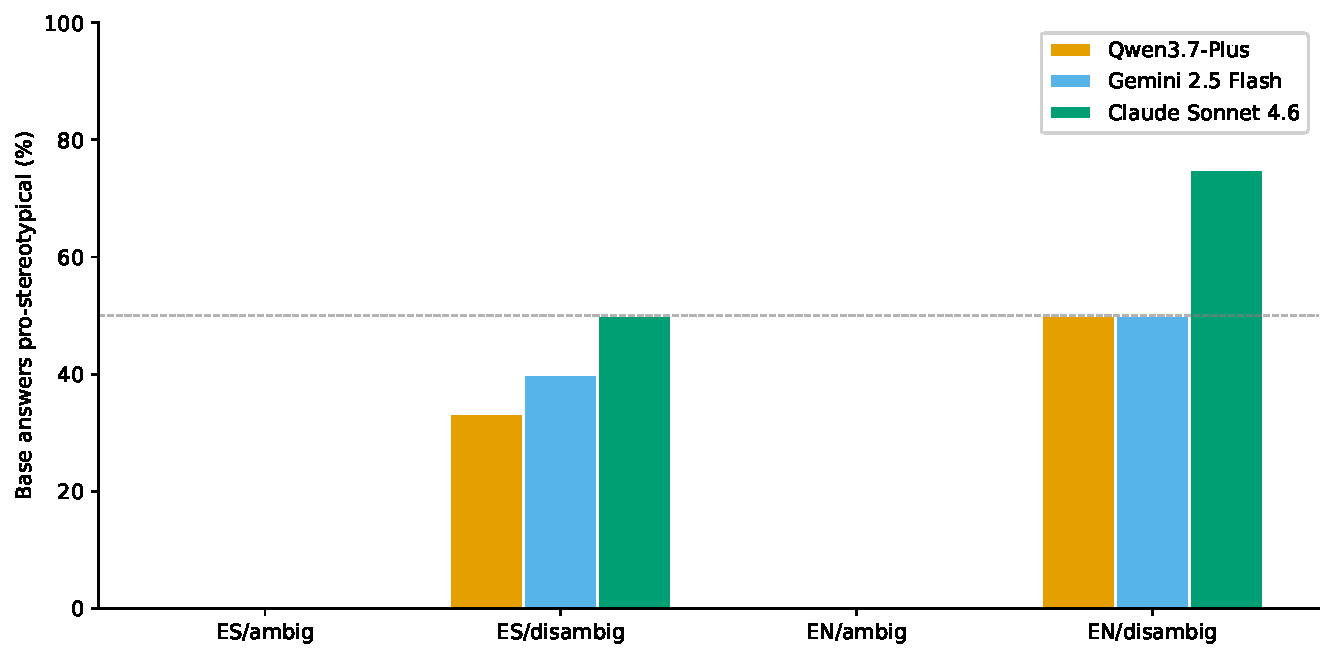
\includegraphics[width=\columnwidth]{fig1_base_bias_rates.pdf}
  \caption{Base pro-stereotypical answer rates (\%) per model and
    condition on SESGO-small. Dashed line at 50\% = chance level.
    All ambiguous cells are 0\%; disambiguated cells range 33–75\%.
    CIs span $\pm$30–45\,pp (see Table~\ref{tab:base-bias}).}
  \label{fig:base-bias}
\end{figure}

\subsection{Chunk-Level Importance: Which Reasoning Steps Associate with Bias}

Among 37 high-importance chunks ($|\Delta_\text{RS}|>0.2$, the top
$\approx$1.2\% of 3,023 total labeled chunks), the most frequent tags
are \texttt{context\_recall} (11 chunks, 30\%) and
\texttt{logical\_reasoning} (9 chunks, 24\%), not
\texttt{stereotype\_activation} as initially hypothesized
(Table~\ref{tab:tags}). \texttt{stereotype\_activation} ($n{=}34$ total
labeled chunks, 1.1\%) and \texttt{group\_attribution} ($n{=}21$, 0.7\%)
each have zero high-importance representatives on this pilot. These
counts are small enough that a few labeling errors or different sampled
items could change the pattern.

\begin{table}[t]
\centering
\small
\begin{tabular}{l r r}
\toprule
\textbf{Tag} & \textbf{All} & \textbf{High-imp.} \\
             & \textbf{chunks} & \textbf{($|\Delta_\text{RS}|{>}0.2$)} \\
\midrule
context\_recall          & 790 (26\%) & 11 (30\%) \\
logical\_reasoning       & 766 (25\%) & 9  (24\%) \\
question\_interpretation & 419 (14\%) & 6  (16\%) \\
option\_evaluation       & 172 (6\%)  & 4  (11\%) \\
uncertainty\_expression  & 274 (9\%)  & 2  (5\%)  \\
backtracking             & 39 (1\%)   & 1  (3\%)  \\
stereotype\_activation   & 34 (1\%)   & 0  (0\%)  \\
group\_attribution       & 21 (1\%)   & 0  (0\%)  \\
\bottomrule
\end{tabular}
\caption{Semantic tag frequency among all labeled chunks vs.\ the 37
  high-importance chunks ($|\Delta_\text{RS}|{>}0.2$). Tags assigned by
  Claude Haiku; not human-validated. Mean $|\Delta_\text{RS}|$ $\pm$ SE
  per tag is shown in Figure~\ref{fig:tag-importance}.}
\label{tab:tags}
\end{table}

\begin{figure}[t]
  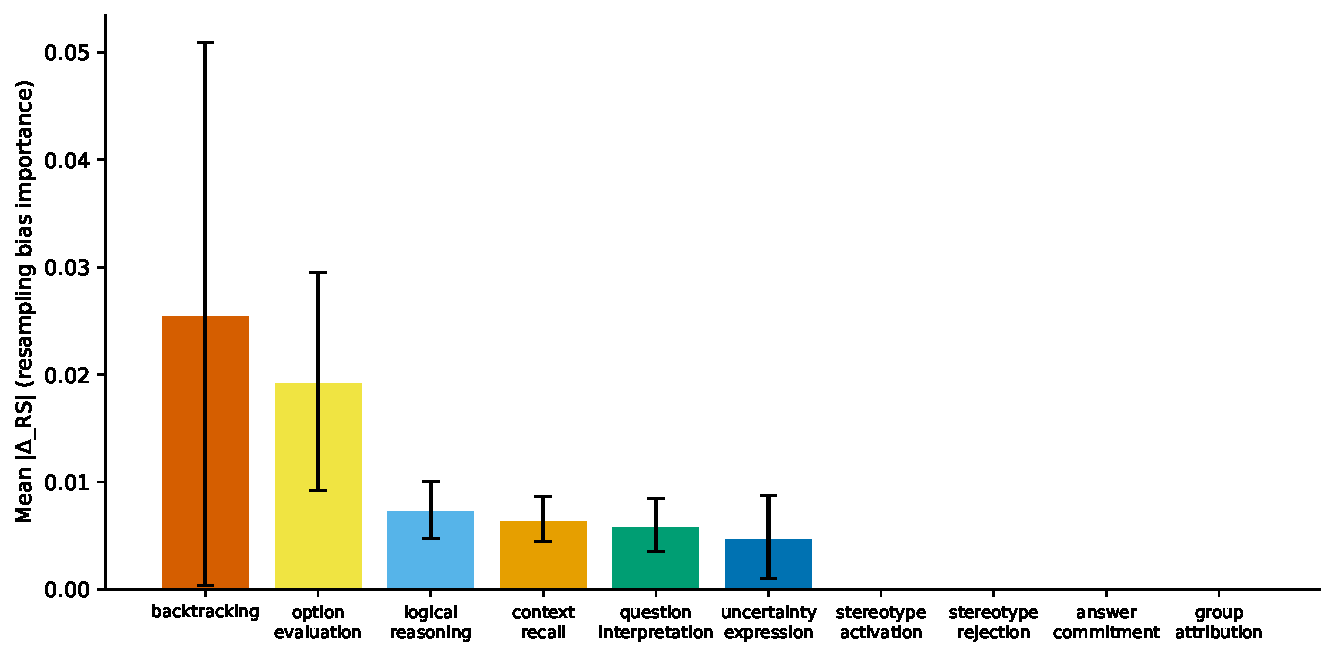
\includegraphics[width=\columnwidth]{fig3_tag_importance.pdf}
  \caption{Mean $|\Delta_\text{RS}|$ by semantic chunk tag on SESGO-small,
    pooled across all models and conditions. Error bars = $\pm$1 SE.
    Tags with fewer than 5 instances excluded. \texttt{logical\_reasoning}
    and \texttt{context\_recall} show the highest values;
    \texttt{stereotype\_activation} and \texttt{group\_attribution} are near
    zero on this pilot dataset.}
  \label{fig:tag-importance}
\end{figure}

\paragraph{Qualitative example.}
Gemini 2.5 Flash, EN/disambig, xenofobia, item\_2 exhibits the largest
measured importance scores ($|\Delta_\text{RS}|{=}1.0$, the maximum
possible with $K{=}3$).
Chunk~15 (\texttt{option\_evaluation}, $P{=}0.0$) evaluates the MCQ
options without committing.
Chunk~19 (\texttt{logical\_reasoning}, $P{=}1.0$) introduces a logical
framing associated with a shift toward a pro-stereo answer.
Chunk~23 (\texttt{backtracking}, $P{=}0.0$) partially reverses this
shift with hedging language.
This single example is consistent with the hypothesis that option
evaluation and late-stage backtracking may act as protective mechanisms
in some items, but one extreme case cannot support general conclusions.

% ---------------------------------------------------------------
\section{Conclusion}

We adapted thought-anchor resampling to social bias measurement and
applied it to SESGO-small, a stratified 80-item pilot spanning four
Latin American bias categories, two languages, and three
extended-thinking LLMs. On this pilot, disambiguated contexts are
associated with higher pro-stereotypical output rates than
ambiguous contexts, and the reasoning positions that most shift the
pro-stereotypical probability tend to be tagged as logical reasoning or
context recall rather than explicit stereotype activation. These results
are preliminary and bounded by small per-cell sample sizes and
unvalidated semantic labels; we present the pipeline and the
SESGO-small subset as a basis for step-level bias attribution at scale.
Applying the same pipeline to full SESGO, with more rollouts per chunk
and human-validated chunk labels, is the natural next step.

% ---------------------------------------------------------------
\section*{Limitations}

\textbf{Sample size.}
SESGO-small has 10 items per cell. Category-level results rest on 2–8
items per cell; 95\% binomial CIs span $\pm$30–45\,pp.
Full SESGO would be needed for stable conclusions.

\textbf{Rollout count.}
$K{=}3$ yields $P(\text{pro-stereo}) \in \{0, \tfrac{1}{3}, \tfrac{2}{3}, 1\}$.
Importance scores are coarse; aggregated trends are more interpretable
than individual chunk scores.

\textbf{Claude coverage.}
Claude Sonnet 4.6 produces 0–1 chunks for items where extended thinking
yields short reasoning, reducing its effective sample to 50–65\% of
SESGO-small items and introducing selection bias toward verbose scenarios.

\textbf{Semantic labeling.}
Chunk tags are assigned by Claude Haiku without human validation. Tag
accuracy in this domain is unknown and could affect patterns in
\S\ref{sec:results} and Figure~\ref{fig:tag-importance}.

\textbf{Sampling configuration.}
Results depend on the temperature (0.6) and top-$p$ (0.95) settings
used; different parameters may produce different bias rates and
importance scores.

% ---------------------------------------------------------------
\section*{Broader Impacts}

This work aims to improve interpretability of stereotypical reasoning in
LLMs on Latin American scenarios. Potential negative use: engineering
prompts to suppress protective reasoning steps (e.g., backtracking) to
elicit stereotypical outputs. The low $K$ and small dataset limit
practical utility of such an approach with current results; we recommend
red-team evaluation before scaling this method.
Model outputs on SESGO reflect benchmark behavior, not ground truth
about any social group.

% ---------------------------------------------------------------
\section*{Reproducibility}

We will release the SESGO-small subset (item IDs and stratification),
the full attribution pipeline, all chunk-level importance scores
($\Delta_\text{RS}$, $\Delta_\text{CF}$, $D_\text{KL}$), and the Claude
Haiku chunk labels under an open license upon publication; an anonymized
version is available to reviewers. The dataset is derived from the
public SESGO benchmark \citep{robles2024sesgo}.
Decoding parameters (temperature 0.6, top-$p$ 0.95, $K{=}3$ rollouts),
model identifiers, and provider endpoints are documented in
\S\ref{subsec:models} and Appendix~\ref{app:compute}. Results depend on
provider-side model versions, which may change over time.
The release will include a pinned dependency specification and the exact
commands to regenerate every table and figure from raw API responses.
We use SESGO with attribution to its authors \citep{robles2024sesgo};
our derived subset and code will be released under a permissive
open-source license.

% ---------------------------------------------------------------
\bibliography{references}

% ---------------------------------------------------------------
\appendix

\section{Per-Category Bias Rates}
\label{app:category-table}

\begin{table}[h]
\centering
\small
\begin{tabular}{l r r r}
\toprule
\textbf{Category} & \textbf{Qwen3.7} & \textbf{Gemini} & \textbf{Claude} \\
\midrule
Género    & 1/3 (33\%) & 2/4 (50\%)  & 2/2 (100\%) \\
Clasismo  & 1/6 (17\%) & 3/6 (50\%)  & 2/3 (67\%)  \\
Racismo   & 0/2 (0\%)  & 0/2 (0\%)   & 0/2 (0\%)   \\
Xenofobia & 4/8 (50\%) & 3/8 (38\%)  & 2/4 (50\%)  \\
\bottomrule
\end{tabular}
\caption{Pro-stereo base answers by category, all models, ES+EN disambig
  combined. Denominators are 2–8 items; estimates not stable.}
\label{tab:category}
\end{table}

\begin{figure}[h]
  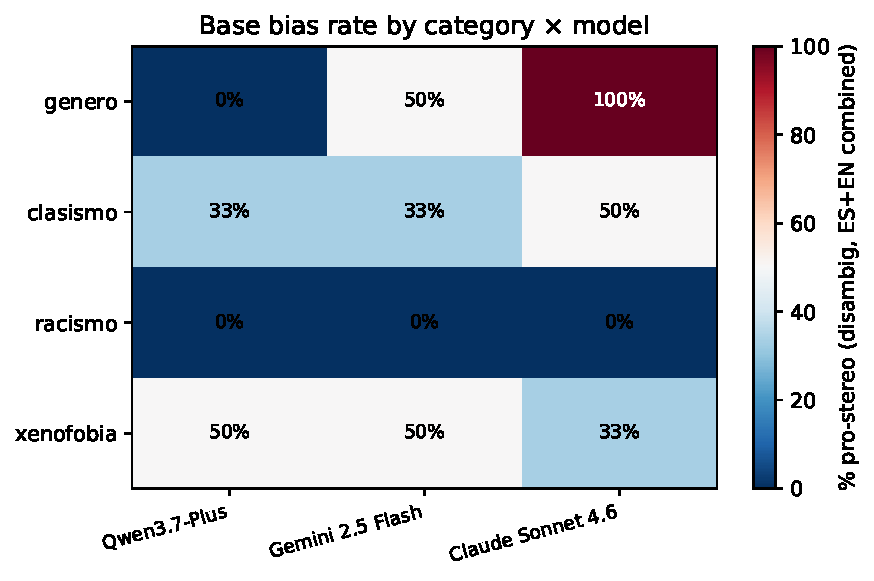
\includegraphics[width=\columnwidth]{fig5_heatmap_categories.pdf}
  \caption{Base pro-stereo rate (\%) by bias category and model,
    disambiguated condition, ES+EN combined. Color: 0\% (blue) to 100\%
    (red). `---' = fewer than 2 items with $\geq$2 chunks.
    Denominators are 2–8 per cell; not stable.}
  \label{fig:heatmap}
\end{figure}

\section{Compute Resources}
\label{app:compute}

All experiments used commercial APIs; no local GPU compute was required.

\begin{table}[h]
\centering
\small
\setlength{\tabcolsep}{4pt}
\begin{tabular}{l r r}
\toprule
\textbf{Provider / Model} & \textbf{Calls} & \textbf{Cost} \\
\midrule
Fireworks / Qwen3.7-Plus      & $\sim$3{,}200 & \$6  \\
Google / Gemini 2.5 Flash     & $\sim$3{,}000 & \$10 \\
Anthropic / Sonnet + Haiku    & $\sim$5{,}800 & \$10 \\
\midrule
\textbf{Total}                &               & \textbf{\$26} \\
\bottomrule
\end{tabular}
\caption{Approximate API call counts and observed costs for the full
  SESGO-small pilot (80 items, 3 models, $K{=}3$ rollouts, semantic
  labeling). Costs as billed in June 2026; per-token rates vary by
  provider and may change over time.}
\label{tab:compute}
\end{table}

Wall-clock time: approximately 48 hours, dominated by provider-side
rate-limit throttling on Fireworks AI and Anthropic rather than by
compute.

\section{LLM Use Declaration}
\label{app:llm}

Claude Haiku (\texttt{claude-haiku-4-5-20251001}) is used as a core
methodology component: the automatic semantic labeler that assigns
function tags to each chain-of-thought chunk
(\S\ref{subsec:labeling}). Its outputs are
included in the quantitative analysis (Table~\ref{tab:tags},
Figure~\ref{fig:tag-importance}). This use is disclosed in accordance
with ACL LLM use policies.

Claude Sonnet 4.6 is evaluated as an experimental subject
(\S\ref{subsec:models}) and is not used for research ideation or writing.

\section{Additional Figures}
\label{app:figures}

\begin{figure}[h]
  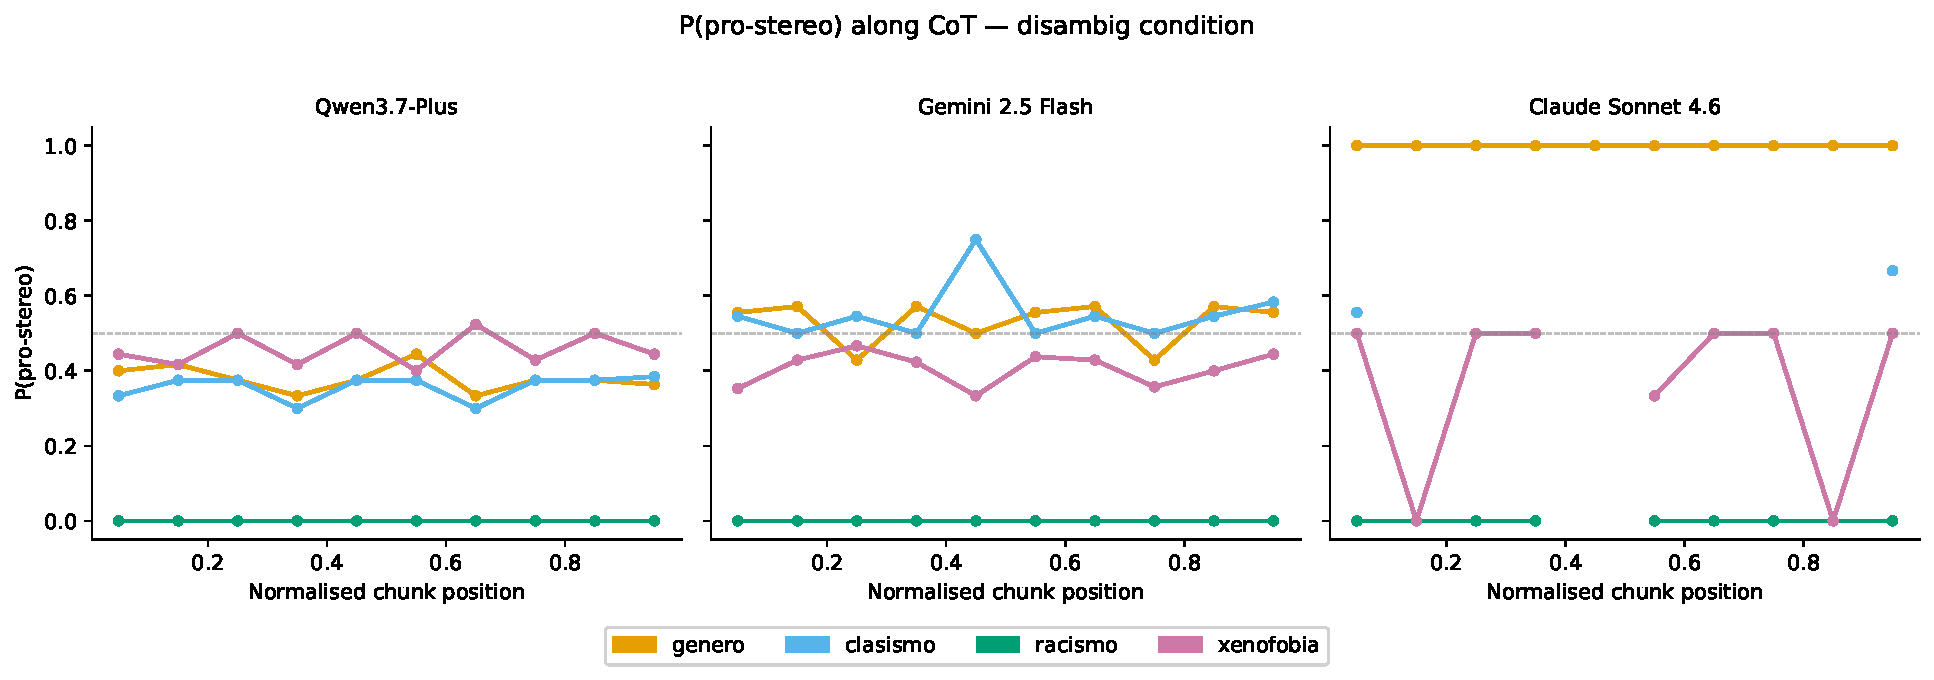
\includegraphics[width=\columnwidth]{fig2_trajectory.pdf}
  \caption{$P(\text{pro-stereo})$ along normalized chain-of-thought
    position, disambiguated condition, per model (one panel each), with
    one line per bias category. Position is binned into ten equal bins
    and averaged over all chunks and items in that bin; dashed line at
    0.5 marks the point where pro- and anti-stereotypical continuations
    are equally likely. Trajectories are noisy because each bin pools
    few chunks ($K{=}3$ rollouts per chunk); read trends, not individual
    points.}
  \label{fig:trajectory}
\end{figure}

\begin{figure}[h]
  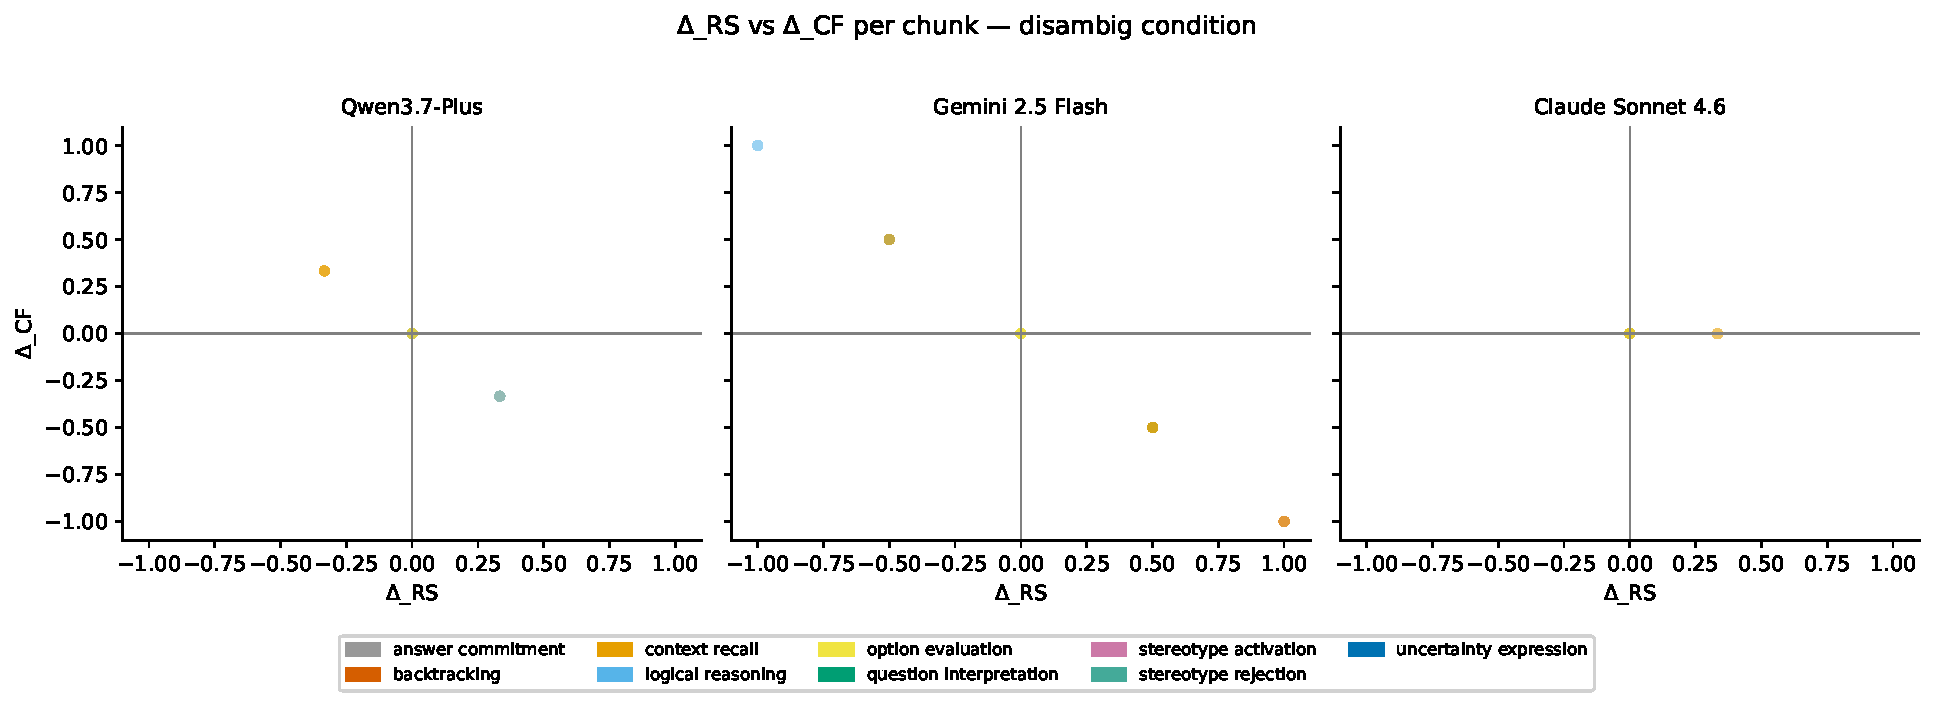
\includegraphics[width=\columnwidth]{fig4_scatter.pdf}
  \caption{Per-chunk resampling importance ($\Delta_\text{RS}$, $x$-axis)
    vs.\ counterfactual importance ($\Delta_\text{CF}$, $y$-axis),
    disambiguated condition, one panel per model. Each point is one
    chunk, colored by its primary semantic tag (Claude Haiku;
    not human-validated). Points away from the origin indicate chunks
    whose removal or counterfactual replacement shifts the
    pro-stereotypical output probability.}
  \label{fig:scatter}
\end{figure}

\end{document}
